\chapter{Experimental Results}\label{ch:exp-result}
\section{Introduction}\label{sec:exp-intro}
In this chapter we will present the experiments we have done in order to study the effects of our repair procedures on the performances of the learning model. We will explain the choices we have done in the design of the experiments, the experimental protocol and then we will show the results we have obtained.
The measure of performances in the prosthetic domain is almost always done in experiment with human participants: given my inexperience in human subject research, all the choices for the experiment design and the results analysis are based on \cite{de2017human}.
%
%
%
%
%
\section{Experiment Design}\label{sec:exp-design}
To compare the performances of the original learning model and of the repaired models we have chosen to do two different experiments: the only difference between the two experiments is given by the value of a single parameter, therefore we have chosen to present the design of the two experiment at the same time.
Both our experiments are instances of the Target Achievement Control (TAC) test for prosthetic hands [\cite{simon2011target}], in which the participant is asked to have a virtual upper limb match a feasible target configuration of the same limb which is visually presented to the participant, from now on we will call a single instances of this kind of test \textit{task}.
In our cases each participants will need to perform a series of tasks using the standard myocontroller, one repaired using the SMT-Repair procedure and one repaired using the PDO-Repair procedure.
Given the time we had to carry out the experiments and the need to keep contained the number of participant required for the results analysis we decided to follow the \textbf{within-subject design} for our experiment, e.g. each participant need to complete a set of task \textit{on each controller}. The results yielded from an experiment using the within-subject design are susceptible to order and carryover effect, therefore is necessary to implement counterbalancing. Counterbalancing aims to keep under control order and carryover effect by letting the participants undergo the various conditions in different orders: in our case the participant will complete the task on the different learning machines in various order. For example the first participant will complete the set of task in a certain order first on the unrepaired controller and then on the other machines, whereas another participant will undergo the same set of task in a different order first on the SMT-Repaired controller and then on the other machines.
In order to avoid that knowledge about the experiment could modify the performances of the participants in the experiment we decided to use \textbf{masking}, e.g. the participants didn't know that they were performing on different controllers and, as consequence, they didn't know which controller were using at any time.
\subsection{Experimental Setup}\label{subsec:exp-setup}
The experimental setup was common to both the experiments: it consisted of a Myo bracelet (see section \ref{sec:interactivemyocontrol}) and two 3D hand models displayed on a computer screen. This two hand model realistically mimic the motions of a human wrist and hand: one is used to provide the visual reference, e.g. it is controlled by the software, whereas the other is used to show the predicted motions as provided by the bracelet and by the chosen controller. We call the first hand model \textit{Stimulus} and the second one \textit{Prosthesis}.
\subsection{Participants}\label{subsec:exp-participants}
As participants for the first experiment we found six intact humans, of which one was female and the others were males, all between 21 and 32 years old. In the other experiment we had twelve intact humans as participants, four were females and six were males, all between 23 and 27 years old. Before beginning the experiment, we clearly explained to each participant, both orally and in writing, that no health risk was involved in the experiment.  Each participant signed an informed consent form. The experiment was previously approved by the internal committee for data protection of the Institution where the experiments took place, and it followed the World Medical Association’s Declaration of Helsinki. All the participant were inexpert users of the system.
\subsection{Experiment Parameters}\label{subsec:exp-parameters}
For both experiments we chose a tolerance threshold of 15\% for the goal to be reached, 1.5 seconds for the required target dwelling time and 15 seconds for the timeout time. In the second experiment we dampened the prediction $f_A$ in order to hopefully elicit overshooting: when the participant would try to reach the maximum activation for $t_A = 1$ they would only see a prediction equals to $f_A = 0.75$ and therefore she would be encouraged to increase her force to $t_A > 1$.  
%
%
%
%
%
\section{Experimental Protocol}\label{sec:exp-protocol}
To each participant was assigned a series of 36 TAC tasks (i.e., hand/wrist configuration to mimic on the screen) on the three different controllers (Unrepaired, SMT-Repaired, PDO-Repaired), therefore each participant needed to complete 12 TAC tasks using each one controller. The tasks covered the three active action of interest: power grasp, wrist flexion and wrist extension; clearly the number of task for each action and for each controller is the same (e.g. 4 tasks for each action and for each machine).
In order to achieve counterbalancing (see section \ref{sec:exp-design}) the order of both the tasks and the controllers was randomised for each participant, whereas the number and type of task was the same for each participant.
In either experiments the participant sat comfortably in front of the computer screen with the Myo bracelet wrapped around her forearm. She was instructed to keep her forearm with an angle of 45 degree and her elbow resting on the armrest.
We then explained to the participant that she would be required to complete a training session for the prosthesis before facing a series of 36 task, during which she would be required to guide the Prosthesis in following the reference shown by the Stimulus as close as possible using the signal from the movements of her own arm.
At the beginning of the training session the Stimulus was shown on the screen and we explained to the participant that the Stimulus would perform a series of movement and that she should mimic what the Stimulus was doing with her own arm. At the end of the explanation the data gathering phase began: the Stimulus played once each action of interest (rest, RE; power grasp, PW; wrist extension, EX; wrist flexion, FL) and while the participant followed the movements of the Stimulus the observation were collected. After the end of the previous phase the Prosthesis would appear on the screen and the series of 36 task would began.
%
%
%
%
%
\section{Experimental Results}\label{sec:exp-results}
\subsection{Performance Measures and Statistics}\label{subsec:measures}
For each task we decided to report the following measures of performance:
\begin{itemize}
    \item \textbf{Success Rate} (\textbf{SR}): this measure is the fraction of task successfully completed, an instance of this measure is computed for each participant as the number of tasks completed successfully by the participant divided for the total number of tasks faced by that participant. This measure is computed separately for each participant and the statistical tests and computations consider the participants as samples.
    \item \textbf{Reaching Rate} (\textbf{RR}): this measure is the fraction of time during which the output $f_A$ was higher than the minimum acceptable value, e.g. the percentage of time the participant actually managed to reach the desired activation value.
    We chose to consider this measure in order to verify whether a failure was really due to overshooting or due to another problem like interference.
    This measure is computed separately for each task and the statistical tests and computations consider the tasks as samples.
    \item \textbf{Time to Complete Task} (\textbf{TCT}): this measure is the time needed to complete a task. This measure is computed separately for each task and the statistical tests and computations consider the tasks as samples.
    \item \textbf{Time In Target} (\textbf{TIT}): this measure is the total time the participant managed to stay in the target before the timeout or before the completion of the task. This measure is computed separately for each task and the statistical tests and computations consider the tasks as samples.
    \item \textbf{Time To Repair} (\textbf{TTR}): this measure is the time needed for the repair process to modify the original controller. This measure is computed separately for each participant because the training and repair of the controller is done one time for each participant and the statistical tests and computations consider the participants as samples.
\end{itemize}
In the following boxplots the central mark represent the median, whereas the upper and the lower edges of the box denotes respectively the 25th and 75th percentiles. The whiskers extend to the extreme data points not considered outliers, whereas the outliers are represented individually using the '$+$' symbol.
As statistical tests for significance we have used the Wilcoxon's Signed Rank test and we have computed the effect size using Cohen's $d$ coefficient.
%
%
%
%
%
\subsection{First Experiment}\label{subsec:first-exp}
In the following we show the above mentioned measures of performance for each of the three controller we have considered (Unrepaired, SMT-Repaired, PDO-Repaired) obtained by the participants of the first experiment: we consider separately each of the measures of interest.
%
%
%
%
%
\subsubsection{Success Rate (SR)}\label{subsub:first-SR}
\begin{table}[ht]
    \centering
    \begin{tabular}{|c|c|c|c|}
        \hline
        - & \textbf{Unrepaired} & \textbf{SMT-Repaired} & \textbf{PDO-Repaired} \\
        \hline
        \textbf{Mean} & 66.67\% & 79.17\% & 63.89\% \\
        \textbf{Standard Deviation} & 19.00\% & 23.42\% & 20.18\% \\
        \hline
    \end{tabular}
    \caption{Table showing the mean and standard deviation of the Success Rate for the different controllers of interest.}
    \label{tab:SR-first-mean-std}
\end{table}
\begin{figure}[ht]
    \centering
    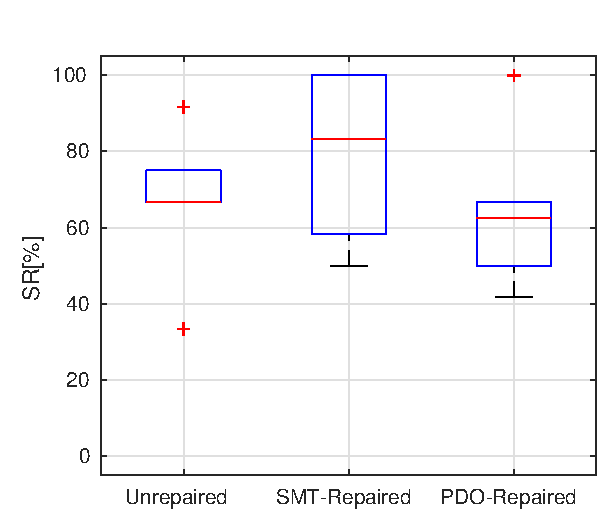
\includegraphics[width=\textwidth]{Images/first-experiment/exp0_success_rate}
    \caption{Boxplot showing the Success Rate (SR) of the participants of the first experiment for the controllers of interest}
    \label{fig:box-SR-first}
\end{figure}
\begin{table}[ht]
    \centering
    \begin{tabular}{|c|c|c|}
        \hline
        - & \textbf{Cohen's} $\mathbf{d}$ & $\mathbf{p-value}$ \\
        \hline
        \textbf{Unrepaired / SMT-Repaired} & 0.5861 & 0.2500 \\
        \textbf{Unrepaired / PDO-Repaired} & 0.1417 & 0.8125 \\
        \textbf{SMT-Repaired / PDO-Repaired} & 0.6988 & 0.2500 \\
        \hline
    \end{tabular}
    \caption{Table showing the Cohen's $d$ coefficient and the p-value of the Success Rate for the different combinations of the controllers of interest.}
    \label{tab:SR-first-cohen-p}
\end{table}
As can be seen from the tables \ref{tab:SR-first-mean-std} and \ref{tab:SR-first-cohen-p} and figure \ref{fig:box-SR-first} there is no statistical significance between the Success Rate of the different machine learned controllers. Even so, considering the values of means and standard deviations, we believe that, given a higher number of participant for the experiment, the difference between the performances of the Unrepaired and the SMT-Repaired controllers would became significant. Anyway the above mentioned results show that the performance of the two repaired controllers are, at least, not inferior to those of the unrepaired one. Another interesting point is that the repaired controllers are the only ones on which at least a participant managed to complete successfully all the tasks. As it could be expected there is no significance between the two repaired controllers.
%
%
%
%
%
\subsubsection{Reaching Rate (RR)}\label{subsub:first-RR}
For the Reaching Rate we have decided to first analyse separately the measurements from the failed task and those from the successful task; then we also analysed the measurements from all the task, both failed and successful, in order to be able to compute the cohen's $d$ coefficient and the p-value.\\
%
%   FAILED
%
\begin{table}[H]
    \centering
    \begin{tabular}{|c|c|c|c|}
        \hline
        - & \textbf{Unrepaired} & \textbf{SMT-Repaired} & \textbf{PDO-Repaired} \\
        \hline
        \textbf{Mean} & 14.61\% & 31.94\% & 30.05\% \\
        \textbf{Standard Deviation} & 62.99\% & 77.06\% & 78.52\% \\
        \hline
    \end{tabular}
    \caption{Table showing the mean and standard deviation of the Reaching Rate for the failed tasks for the different controllers of interest.}
    \label{tab:RR-fail-first-mean-std}
\end{table}
\begin{figure}[H]
    \centering
    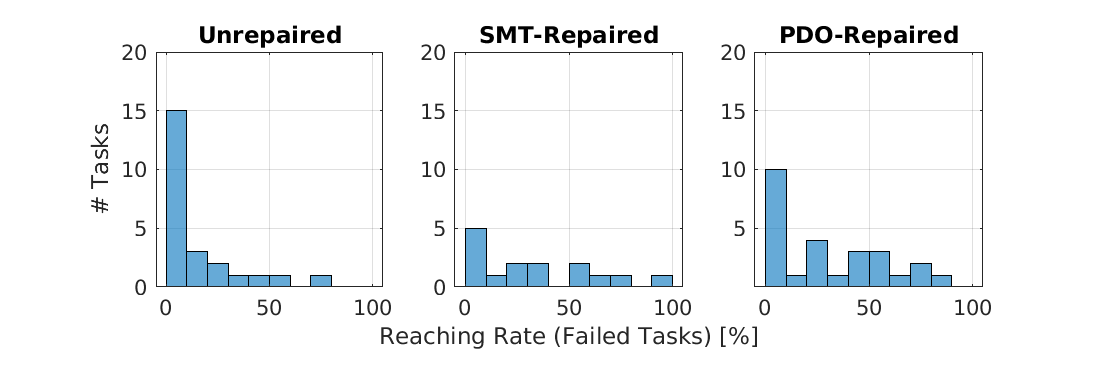
\includegraphics[width=\textwidth]{Images/first-experiment/exp0_RR_fail_hist.eps}
    \caption{Histogram showing the number of failed tasks for Reaching Rate (RR) for the first experiment for the controllers of interest}
    \label{fig:hist-RR-fail-first}
\end{figure}
\begin{figure}[H]
    \centering
    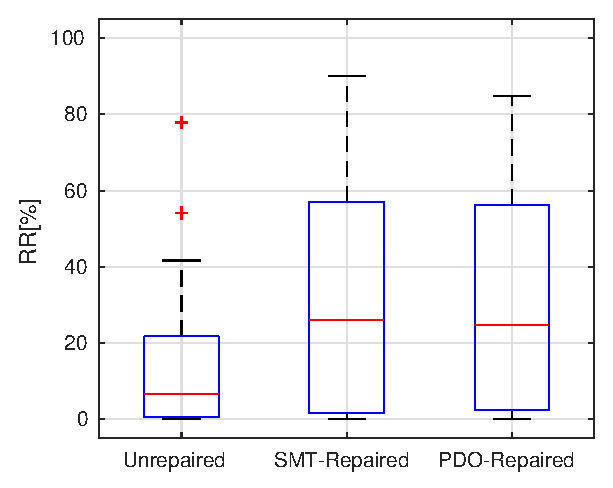
\includegraphics[width=\textwidth]{Images/first-experiment/exp0_RR_fail_box.eps}
    \caption{Boxplot showing the Reaching Rate (RR) of the failed tasks of the first experiment for the controllers of interest}
    \label{fig:box-RR-fail-first}
\end{figure}
As can be seen from table \ref{tab:RR-fail-first-mean-std} and figures \ref{fig:hist-RR-fail-first} and \ref{fig:box-RR-fail-first} the reaching rate for the failed tasks is significantly higher for the two repaired controllers: in particular the mean of the reaching rate is more or less twice that of the unrepaired controller. This result show that  even if the participant didn't manage to complete successfully some tasks, it was still easier to reach the correct activation value on the two repaired controllers then on the unrepaired one. Furthermore this result can be seen as the proof that both our automated repair process indeed manage to enhance the reliability of the original controller with respect to the problem of activation overshooting.\\
%
%   SUCCESSFUL
%
\begin{table}[H]
    \centering
    \begin{tabular}{|c|c|c|c|}
        \hline
        - & \textbf{Unrepaired} & \textbf{SMT-Repaired} & \textbf{PDO-Repaired} \\
        \hline
        \textbf{Mean} & 62.99\% & 77.06\% & 78.52\% \\
        \textbf{Standard Deviation} & 19.83\% & 19.39\% & 17.72\% \\
        \hline
    \end{tabular}
    \caption{Table showing the mean and standard deviation of the Reaching Rate for the successful tasks for the different controllers of interest.}
    \label{tab:RR-succ-first-mean-std}
\end{table}
\begin{figure}[H]
    \centering
    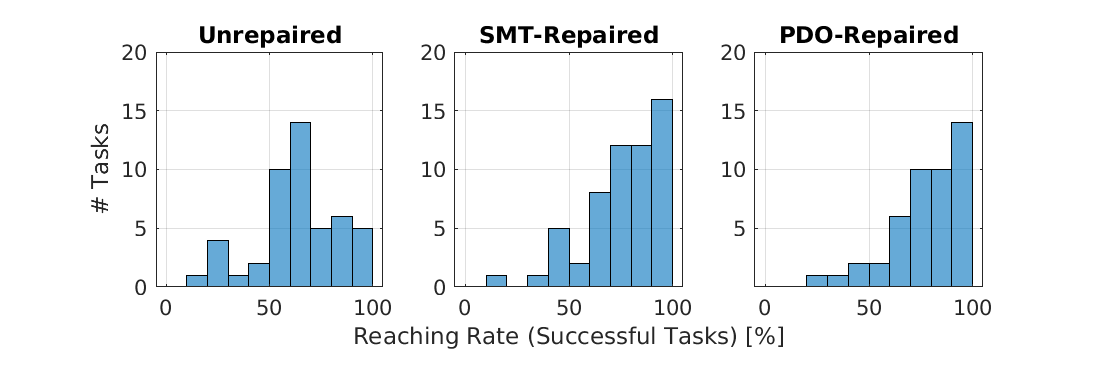
\includegraphics[width=\textwidth]{Images/first-experiment/exp0_RR_succ_hist.eps}
    \caption{Histogram showing the number of successful tasks for Reaching Rate (RR) for the first experiment for the controllers of interest}
    \label{fig:hist-RR-succ-first}
\end{figure}
\begin{figure}[H]
    \centering
    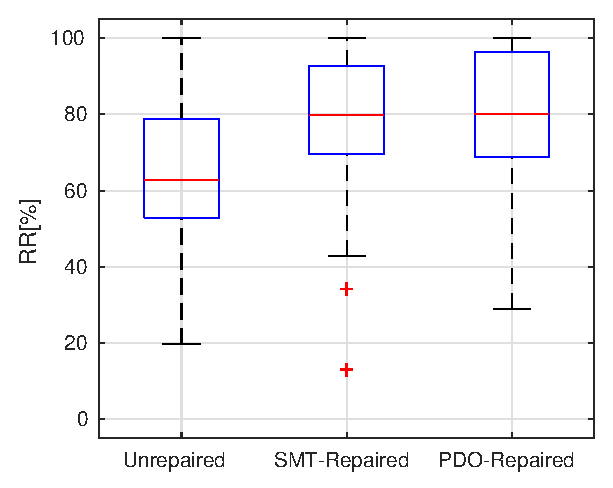
\includegraphics[width=\textwidth]{Images/first-experiment/exp0_RR_succ_box.eps}
    \caption{Boxplot showing the Reaching Rate (RR) of the successful tasks of the first experiment for the controllers of interest}
    \label{fig:box-RR-succ-first}
\end{figure}
In figure \ref{fig:box-RR-succ-first} and \ref{fig:hist-RR-succ-first} and table \ref{tab:RR-succ-first-mean-std} it is possible to see that the results we have found for the failed tasks are valid also for the successful tasks. Therefore we can consider these results as an indication that, even where the task are successful, the repair process manage to make it easier to reach the correct activation value.\\
%
%   ALL
%
\begin{figure}[H]
    \centering
    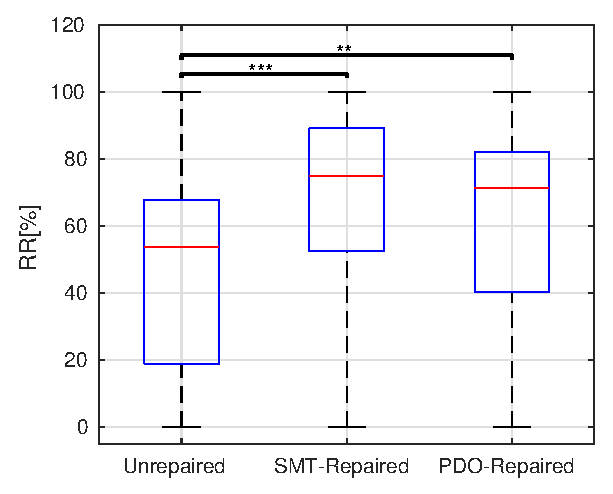
\includegraphics[width=\textwidth]{Images/first-experiment/exp0_RR_all_box.eps}
    \caption{Boxplot showing the Reaching Rate (RR) of all the tasks of the first experiment for the controllers of interest}
    \label{fig:box-RR-all-first}
\end{figure}
\begin{table}[H]
    \centering
    \begin{tabular}{|c|c|c|c|}
        \hline
        - & \textbf{Unrepaired} & \textbf{SMT-Repaired} & \textbf{PDO-Repaired} \\
        \hline
        \textbf{Mean} & 46.86\% & 67.66\% & 61.01\% \\
        \textbf{Standard Deviation} & 30.33\% & 28.58\% & 31.81\% \\
        \hline
    \end{tabular}
    \caption{Table showing the mean and standard deviation of the Reaching Rate for the all the tasks for the different controllers of interest.}
    \label{tab:RR-all-first-mean-std}
\end{table}
\begin{table}[H]
    \centering
    \begin{tabular}{|c|c|c|}
        \hline
        - & \textbf{Cohen's} $\mathbf{d}$ & $\mathbf{p-value}$ \\
        \hline
        \textbf{Unrepaired / SMT-Repaired} & 0.7059 & $2.0509 \cdot 10^{-5}$ \\
        \textbf{Unrepaired / PDO-Repaired} & 0.4553 & 0.0070\\
        \textbf{SMT-Repaired / PDO-Repaired} & 0.2199 & 0.0925 \\
        \hline
    \end{tabular}
    \caption{Table showing the Cohen's $d$ coefficient and the p-value of the Reaching Rate for the different combinations of the controllers of interest.}
    \label{tab:RR-all-first-cohen-p}
\end{table}
\begin{figure}[H]
    \centering
    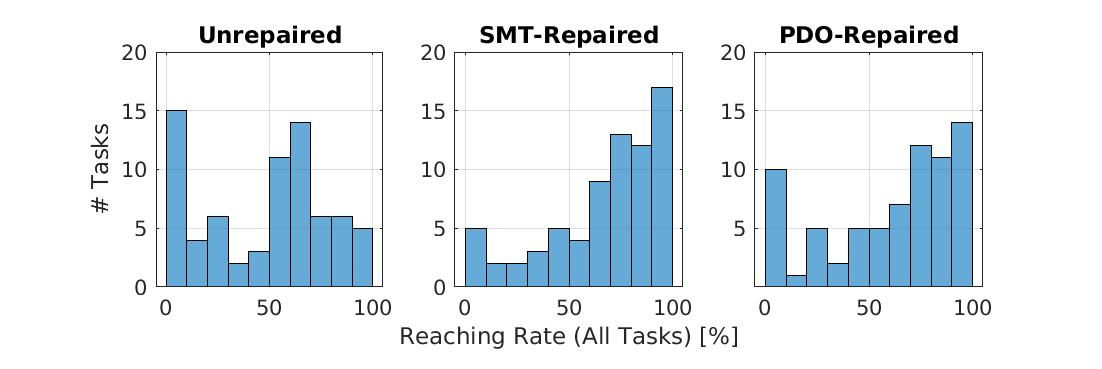
\includegraphics[width=\textwidth]{Images/first-experiment/exp0_RR_all_hist.eps}
    \caption{Histogram showing the number of successful tasks for Reaching Rate (RR) for the first experiment for the controllers of interest}
    \label{fig:hist-RR-all-first}
\end{figure}
As expected the results from the analysis on all the tasks are coherent with what we have found in the previous analysis. The interesting extension of this analysis is that, considering all the tasks, we have the same number of samples for all the three different controllers and therefore we can compute the effect size and the p-value for the different couples of controllers. As can be seen from figure \ref{fig:box-RR-all-first} and table \ref{tab:RR-all-first-cohen-p} there are a medium effect size and a very high significance between the Unrepaired and SMT-Repaired controllers, whereas there are a small effect size and an high significance between the Unrepaired and the PDO-Repaired controllers. There is no significant difference between the two repaired controllers.
%
%
%
%
%
\subsubsection{Time to Complete Task (TCT)}\label{subsub:first-TCT}
We have decided to present the analysis of the TCTs both for only the successful tasks and for all the task together. We decided to do so because the TCTs of the failed tasks saturate at 15 seconds, therefore is not really informative; even so we decided to consider also the failed task in another analysis in order to have the same number of samples for all the three controllers and therefore being able to compute size effect and p-value for all the possible couples of controllers.
\begin{figure}[H]
    \centering
    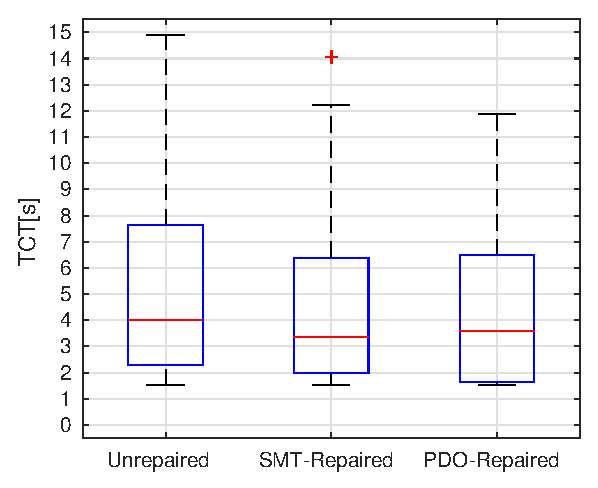
\includegraphics[width=\textwidth]{Images/first-experiment/exp0_TCT_succ.eps}
    \caption{Boxplot showing the Time to Complete Task (TCT) of the successful tasks of the first experiment for the controllers of interest}
    \label{fig:box-TCT-succ-first}
\end{figure}
\begin{table}[H]
    \centering
    \begin{tabular}{|c|c|c|c|}
        \hline
        - & \textbf{Unrepaired} & \textbf{SMT-Repaired} & \textbf{PDO-Repaired} \\
        \hline
        \textbf{Mean} & 5.0287s & 4.3859s & 4.2665s \\
        \textbf{Standard Deviation} & 3.1297s & 3.0237s & 2.5868s \\
        \hline
    \end{tabular}
    \caption{Table showing the mean and standard deviation of the Time to Complete Task for the successful tasks for the different controllers of interest.}
    \label{tab:TCT-succ-first-mean-std}
\end{table}
\begin{figure}[H]
    \centering
    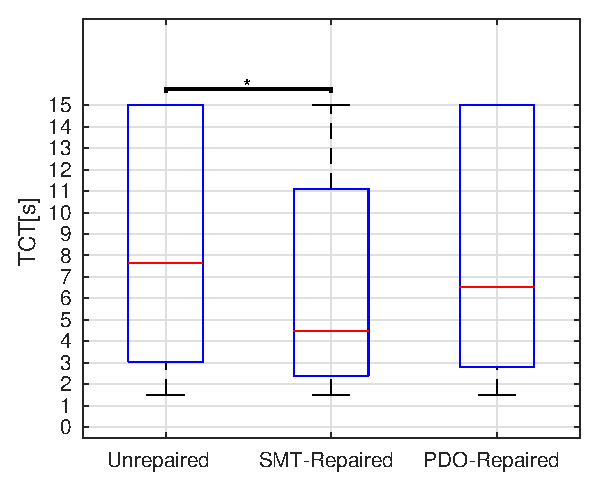
\includegraphics[width=\textwidth]{Images/first-experiment/exp0_TCT.eps}
    \caption{Boxplot showing the Time to Complete Task (TCT) of all the tasks of the first experiment for the controllers of interest}
    \label{fig:box-TCT-all-first}
\end{figure}
\begin{table}[H]
    \centering
    \begin{tabular}{|c|c|c|c|}
        \hline
        - & \textbf{Unrepaired} & \textbf{SMT-Repaired} & \textbf{PDO-Repaired} \\
        \hline
        \textbf{Mean} & 8.3540s & 6.5981s & 8.1443s \\
        \textbf{Standard Deviation} & 5.3769s & 5.1060s & 5.5875s \\
        \hline
    \end{tabular}
    \caption{Table showing the mean and standard deviation of the Time to Complete Task for the all the tasks for the different controllers of interest.}
    \label{tab:TCT-all-first-mean-std}
\end{table}
\begin{table}[H]
    \centering
    \begin{tabular}{|c|c|c|}
        \hline
        - & \textbf{Cohen's} $\mathbf{d}$ & $\mathbf{p-value}$ \\
        \hline
        \textbf{Unrepaired / SMT-Repaired} & 0.3349 & 0.0105 \\
        \textbf{Unrepaired / PDO-Repaired} & 0.0382 & 0.9374\\
        \textbf{SMT-Repaired / PDO-Repaired} & 0.2889 & 0.0819 \\
        \hline
    \end{tabular}
    \caption{Table showing the Cohen's $d$ coefficient and the p-value of the Time to Complete Task for the different combinations of the controllers of interest.}
    \label{tab:TCT-all-first-cohen-p}
\end{table}
As can be seen from figures \ref{fig:box-TCT-succ-first} and \ref{fig:box-TCT-all-first} and tables \ref{tab:TCT-succ-first-mean-std} and \ref{tab:TCT-all-first-mean-std} the TCTs for the SMT-Repaired controller are lower than the other two and in particular they are significantly lower than that of the unrepaired one. From this result we could infer that the SMT-Repaired controller is easier to use then the other two: the participants needed less time to complete the task on the SMT-Repaired controller then on the other controllers. In order to confirm this hypothesis it would be necessary to perform further experiment.
%
%
%
%
%
\subsubsection{Time In Target (TIT)}\label{subsub:first-TIT}
For the analysis of the TITs we decided to consider separately the analysis of the failed tasks and of all tasks. This is because for the successful task the TITs are usually equals to 1.5s (e.g. the required target dwelling time) and therefore are not informative. The analysis of all tasks is justified by the necessity of computing effect sizes and p-values.
\begin{figure}[H]
    \centering
    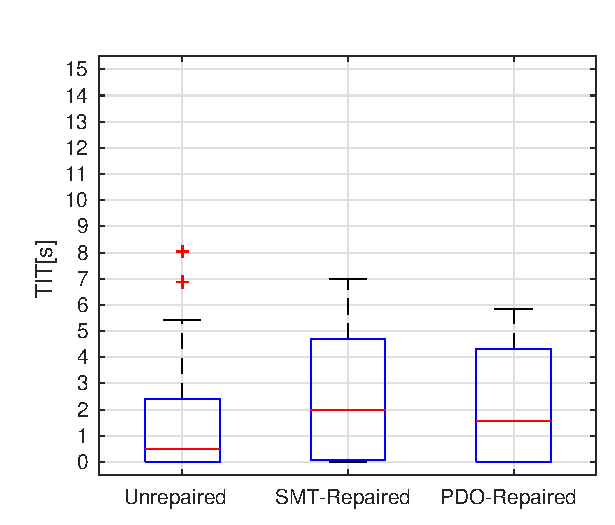
\includegraphics[width=\textwidth]{Images/first-experiment/exp0_TIT_fail.eps}
    \caption{Boxplot showing the Time In Target (TIT) of the failed tasks of the first experiment for the controllers of interest}
    \label{fig:box-TIT-fail-first}
\end{figure}
\begin{table}[H]
    \centering
    \begin{tabular}{|c|c|c|c|}
        \hline
        - & \textbf{Unrepaired} & \textbf{SMT-Repaired} & \textbf{PDO-Repaired} \\
        \hline
        \textbf{Mean} & 1.5511s & 2.3931s & 2.1376s \\
        \textbf{Standard Deviation} & 2.3223s & 2.3328s & 2.2450s \\
        \hline
    \end{tabular}
    \caption{Table showing the mean and standard deviation of the Time In Target for the failed tasks for the different controllers of interest.}
    \label{tab:TIT-fail-first-mean-std}
\end{table}
\begin{figure}[H]
    \centering
    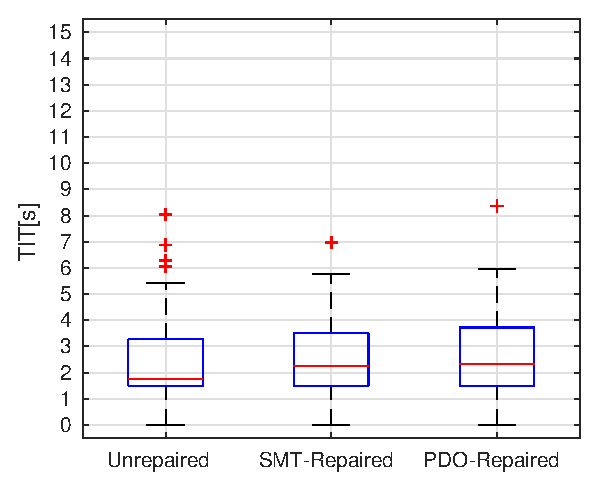
\includegraphics[width=\textwidth]{Images/first-experiment/exp0_TIT.eps}
    \caption{Boxplot showing the Time In Target (TIT) of all the tasks of the first experiment for the controllers of interest}
    \label{fig:box-TIT-all-first}
\end{figure}
\begin{table}[H]
    \centering
    \begin{tabular}{|c|c|c|c|}
        \hline
        - & \textbf{Unrepaired} & \textbf{SMT-Repaired} & \textbf{PDO-Repaired} \\
        \hline
        \textbf{Mean} & 2.2693s & 2.6097s & 2.4885s \\
        \textbf{Standard Deviation} & 1.7874s & 1.5486s & 1.7622s \\
        \hline
    \end{tabular}
    \caption{Table showing the mean and standard deviation of the Time In Target for the all the tasks for the different controllers of interest.}
    \label{tab:TIT-all-first-mean-std}
\end{table}
\begin{table}[H]
    \centering
    \begin{tabular}{|c|c|c|}
        \hline
        - & \textbf{Cohen's} $\mathbf{d}$ & $\mathbf{p-value}$ \\
        \hline
        \textbf{Unrepaired / SMT-Repaired} & 0.2036 & 0.0902 \\
        \textbf{Unrepaired / PDO-Repaired} & 0.1235 & 0.1448\\
        \textbf{SMT-Repaired / PDO-Repaired} & 0.0731 & 0.6714 \\
        \hline
    \end{tabular}
    \caption{Table showing the Cohen's $d$ coefficient and the p-value of the Time In Target for the different combinations of the controllers of interest.}
    \label{tab:TIT-all-first-cohen-p}
\end{table}
As can be seen from figure \ref{fig:box-TIT-all-first} and tables \ref{tab:TIT-all-first-mean-std} and \ref{tab:TIT-all-first-mean-std} there is not a significant difference between the controllers in term of Time In Target. Figure \ref{fig:box-TIT-fail-first} and table \ref{tab:TIT-fail-first-mean-std} hints to higher TITs for the SMT-Repaired machine, which indicates that, even if the participants didn't complete the tasks successfully, they still managed to keep the prediction near the target for a certain time. With what we have seen for the TCTs this fact seems to hint to an higher ease of use for the SMT-Repaired controller.
\subsubsection{Time To Repair (TTR)}\label{subsub:first-TTR}
\begin{figure}[H]
    \centering
    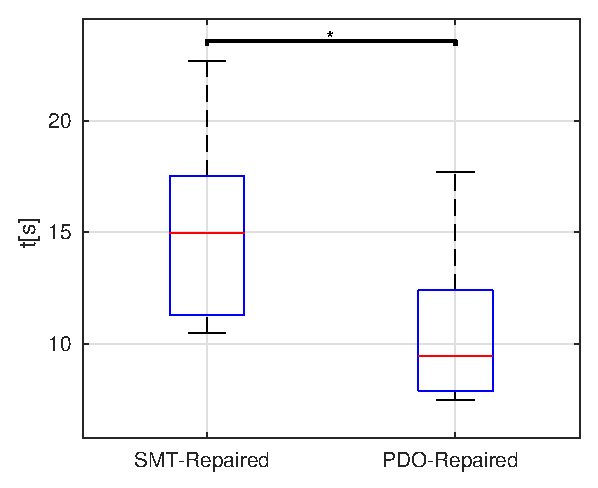
\includegraphics[width=\textwidth]{Images/first-experiment/exp0_time_to_repair.eps}
    \caption{Boxplot showing the Time To Repair (TTR) for all the participants of the first experiment for the controllers of interest}
    \label{fig:box-TTR-first}
\end{figure}
\begin{table}[H]
    \centering
    \begin{tabular}{|c|c|c|}
        \hline
        - & \textbf{SMT-Repaired} & \textbf{PDO-Repaired} \\
        \hline
        \textbf{Mean} & 15.3242s & 10.7226s \\
        \textbf{Standard Deviation} & 4.5760s & 3.9638s \\
        \hline
    \end{tabular}
    \caption{Table showing the mean and standard deviation of the Time To Repair for the all the participants for the different controllers of interest.}
    \label{tab:TTR-first-mean-std}
\end{table}
\begin{table}[H]
    \centering
    \begin{tabular}{|c|c|c|}
        \hline
        - & \textbf{Cohen's} $\mathbf{d}$ & $\mathbf{p-value}$ \\
        \hline
        \textbf{SMT-Repaired / PDO-Repaired} & 1.0749 & 0.0313 \\
        \hline
    \end{tabular}
    \caption{Table showing the Cohen's $d$ coefficient and the p-value of the Time To Repair for the different combinations of the controllers of interest.}
    \label{tab:TTR-first-cohen-p}
\end{table}
As can be seen from figure \ref{fig:box-TTR-first} and tables \ref{tab:TTR-first-mean-std} and \ref{tab:TTR-first-cohen-p} the PDO-Repair process' temporal overhead is lower then that of the SMT-Repair one. There is also a statistical significance between the TTRs of the two controllers and a large effect size. As we would expect, the temporal overhead of the repair process which leverage the SMT solver is higher then the one which only uses statistical methods. However the difference between the two temporal overhead is not so large to clearly define an optimal repair process: the selection between the two process should also consider the stricter guarantee given by the SMT-Repair.
%
%
%
%
%
\subsection{Second Experiment}\label{subsec:second-exp}
In the following we show the above mentioned measures of performance for each of the three controller we have considered (Unrepaired, SMT-Repaired, PDO-Repaired) obtained by the participants of the second experiment: we consider separately each of the measures of interest. We remind that, as seen in subsection \ref{subsec:exp-parameters}, in this experiment we have dampened the predictions $f_{A}$ in order to elicit the activation overshooting.
%
%
%
%
%
\subsubsection{Success Rate (SR)}\label{subsub:second-SR}
\begin{table}[H]
    \centering
    \begin{tabular}{|c|c|c|c|}
        \hline
        - & \textbf{Unrepaired} & \textbf{SMT-Repaired} & \textbf{PDO-Repaired} \\
        \hline
        \textbf{Mean} & 14.58\% & 46.53\% & 45.83\% \\
        \textbf{Standard Deviation} & 21.06\% & 22.88\% & 18.29\% \\
        \hline
    \end{tabular}
    \caption{Table showing the mean and standard deviation of the Success Rate for the different controllers of interest in the second experiment.}
    \label{tab:SR-second-mean-std}
\end{table}
\begin{figure}[H]
    \centering
    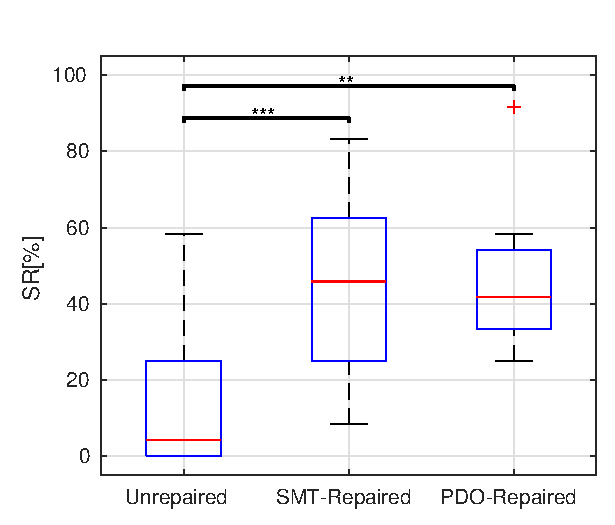
\includegraphics[width=\textwidth]{Images/second-experiment/exp1_success_rate}
    \caption{Boxplot showing the Success Rate (SR) of the participants of the second experiment for the controllers of interest}
    \label{fig:box-SR-second}
\end{figure}
\begin{table}[H]
    \centering
    \begin{tabular}{|c|c|c|}
        \hline
        - & \textbf{Cohen's} $\mathbf{d}$ & $\mathbf{p-value}$ \\
        \hline
        \textbf{Unrepaired / SMT-Repaired} & 1.4528 & $9.7656 \cdot 10^{-4}$ \\
        \textbf{Unrepaired / PDO-Repaired} & 1.5843 & 0.0020 \\
        \textbf{SMT-Repaired / PDO-Repaired} & 0.0335 & 0.8477 \\
        \hline
    \end{tabular}
    \caption{Table showing the Cohen's $d$ coefficient and the p-value of the Success Rate for the different combinations of the controllers of interest in the second experiment.}
    \label{tab:SR-second-cohen-p}
\end{table}
As can be seen from figure \ref{fig:box-SR-second} and tables \ref{tab:SR-second-mean-std} and \ref{tab:SR-second-cohen-p} the Success Rate drastically increase with both the repair processes. Moreover there is a large effect size between the Unrepaired controller and the two repaired ones, the results obtained has also an high statistical significance. These results show that both the repair processes manage to deeply enhance the reliability of the controllers in the \textit{"danger zone"} of the activation overshooting. The general lower value for the Success Rate, with respect to the first experiment, is due to the instability inherent to the high level of muscular activation which brings to other problems like interference.
%
%
%
%
%
\subsubsection{Reaching Rate (RR)}\label{subsub:second-RR}
As in the first experiment, for the Reaching Rate we have decided to first analyse separately the measurements from the failed task and those from the successful task; then we also analysed the measurements from all the task, both failed and successful, in order to be able to compute the cohen's $d$ coefficient and the p-value.\\
%
%   FAILED
%
\begin{figure}[H]
    \centering
    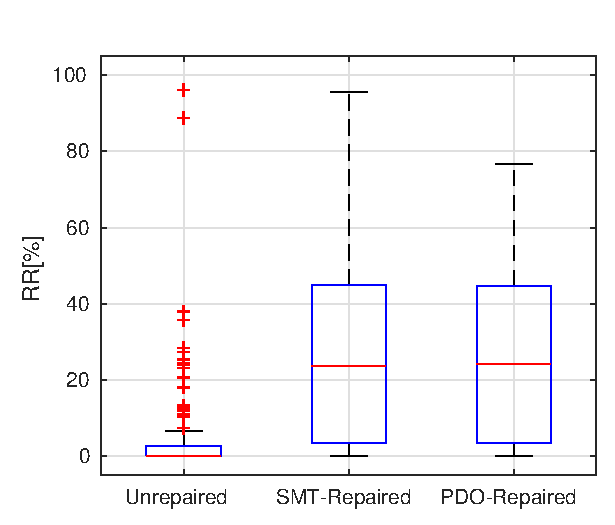
\includegraphics[width=\textwidth]{Images/second-experiment/exp1_RR_fail_box.eps}
    \caption{Boxplot showing the Reaching Rate (RR) of the failed tasks of the second experiment for the controllers of interest}
    \label{fig:box-RR-fail-second}
\end{figure}
\begin{table}[H]
    \centering
    \begin{tabular}{|c|c|c|c|}
        \hline
        - & \textbf{Unrepaired} & \textbf{SMT-Repaired} & \textbf{PDO-Repaired} \\
        \hline
        \textbf{Mean} & 4.96\% & 28.67\% & 26.71\% \\
        \textbf{Standard Deviation} & 13.62\% & 27.80\% & 22.78\% \\
        \hline
    \end{tabular}
    \caption{Table showing the mean and standard deviation of the Reaching Rate for the failed tasks for the different controllers of interest in the second experiment.}
    \label{tab:RR-fail-second-mean-std}
\end{table}
\begin{figure}[H]
    \centering
    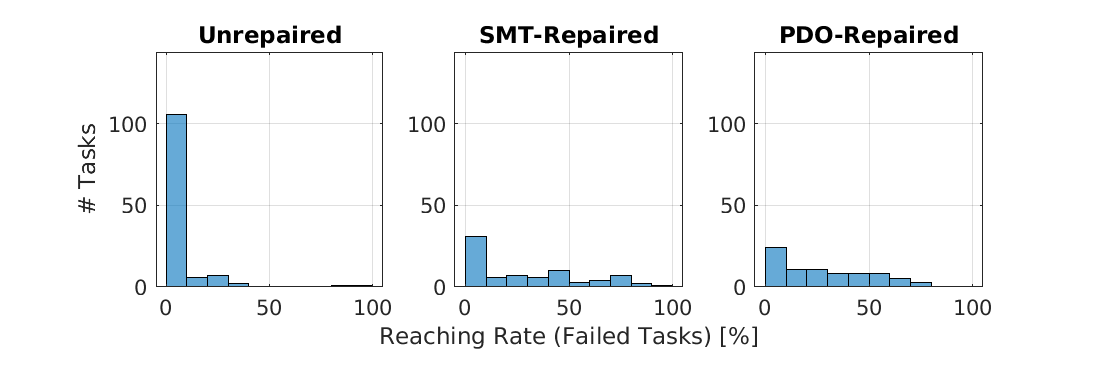
\includegraphics[width=\textwidth]{Images/second-experiment/exp1_RR_fail_hist.eps}
    \caption{Histogram showing the number of failed tasks for Reaching Rate (RR) for the second experiment for the controllers of interest}
    \label{fig:hist-RR-fail-second}
\end{figure}
Figures \ref{fig:hist-RR-fail-second} and \ref{fig:box-RR-fail-second} and table \ref{tab:RR-fail-second-mean-std} show that the Reaching Rates of the failed tasks increase drastically in the repaired controllers: this means that, even if the participants failed the tasks, they still managed to reach the correct activation value for more time using the repaired controllers than using the unrepaired one. 
%
%   SUCCESSFUL
%
\begin{figure}[H]
    \centering
    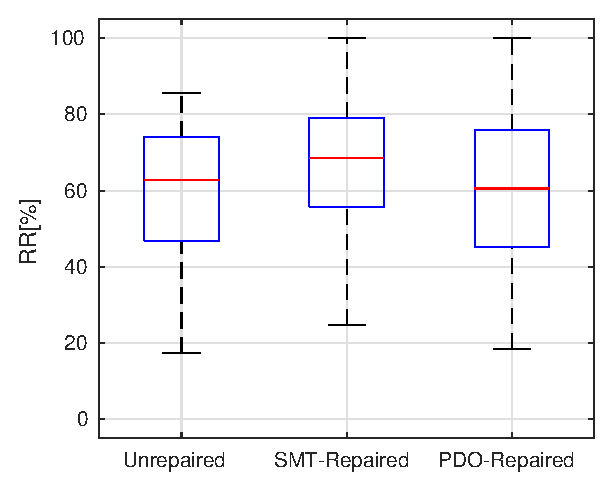
\includegraphics[width=\textwidth]{Images/second-experiment/exp1_RR_succ_box.eps}
    \caption{Boxplot showing the Reaching Rate (RR) of the successful tasks of the second experiment for the controllers of interest}
    \label{fig:box-RR-succ-second}
\end{figure}
\begin{table}[H]
    \centering
    \begin{tabular}{|c|c|c|c|}
        \hline
        - & \textbf{Unrepaired} & \textbf{SMT-Repaired} & \textbf{PDO-Repaired} \\
        \hline
        \textbf{Mean} & 58.48\% & 67.61\% & 61.35\% \\
        \textbf{Standard Deviation} & 19.08\% & 16.43\% & 20.83\% \\
        \hline
    \end{tabular}
    \caption{Table showing the mean and standard deviation of the Reaching Rate for the successful tasks for the different controllers of interest in the second experiment.}
    \label{tab:RR-succ-second-mean-std}
\end{table}
\begin{figure}[H]
    \centering
    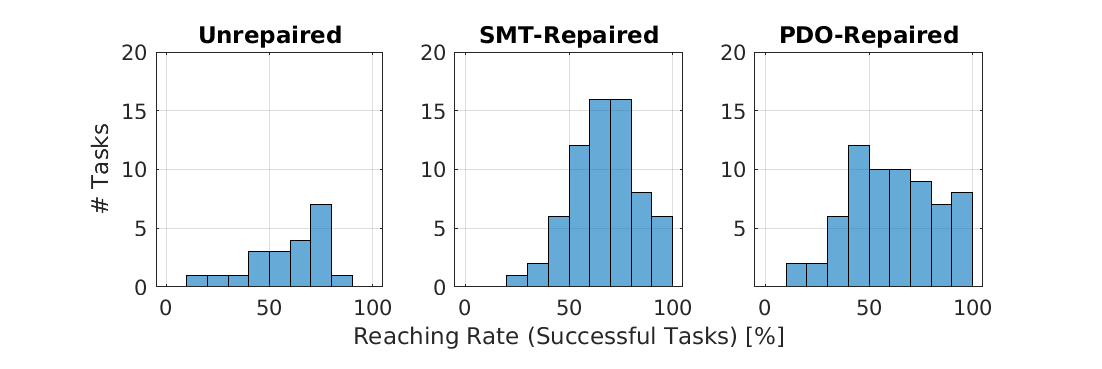
\includegraphics[width=\textwidth]{Images/second-experiment/exp1_RR_succ_hist.eps}
    \caption{Histogram showing the number of successful tasks for Reaching Rate (RR) for the second experiment for the controllers of interest}
    \label{fig:hist-RR-succ-second}
\end{figure}
As can be seen from figures \ref{fig:box-RR-succ-second} and \ref{fig:hist-RR-succ-second} and tables \ref{tab:RR-succ-second-mean-std} the Reaching Rates of the successful task don't differ much between the repaired controller and the unrepaired ones. The fact that the reaching rates are around 60\% indicates that, even when the participants managed to complete successfully the tasks, they still needed some time to arrive and stay in the correct activation value. This is due to the inherent instability of the zone of high muscular activation, in which we bring the participant by eliciting the overshooting.
%
%   ALL
%
\begin{figure}[H]
    \centering
    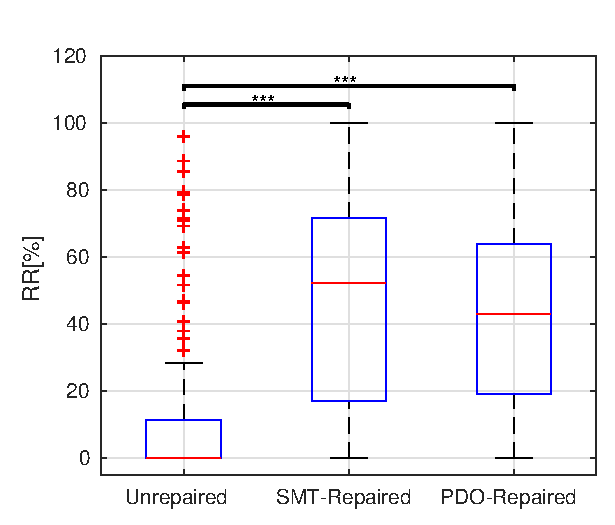
\includegraphics[width=\textwidth]{Images/second-experiment/exp1_RR_all_box.eps}
    \caption{Boxplot showing the Reaching Rate (RR) of all the tasks of the second experiment for the controllers of interest}
    \label{fig:box-RR-all-second}
\end{figure}
\begin{table}[H]
    \centering
    \begin{tabular}{|c|c|c|c|}
        \hline
        - & \textbf{Unrepaired} & \textbf{SMT-Repaired} & \textbf{PDO-Repaired} \\
        \hline
        \textbf{Mean} & 12.76\% & 46.79\% & 42.59\% \\
        \textbf{Standard Deviation} & 23.84\% & 30.26\% & 27.87\% \\
        \hline
    \end{tabular}
    \caption{Table showing the mean and standard deviation of the Reaching Rate for the all the tasks for the different controllers of interest in the second experiment.}
    \label{tab:RR-all-second-mean-std}
\end{table}
\begin{table}[H]
    \centering
    \begin{tabular}{|c|c|c|}
        \hline
        - & \textbf{Cohen's} $\mathbf{d}$ & $\mathbf{p-value}$ \\
        \hline
        \textbf{Unrepaired / SMT-Repaired} & 1.2492 & $6.3945 \cdot 10^{-17}$ \\
        \textbf{Unrepaired / PDO-Repaired} & 1.1501 & $5.0207 \cdot 10^{-15}$ \\
        \textbf{SMT-Repaired / PDO-Repaired} & 0.1445 & 0.1567 \\
        \hline
    \end{tabular}
    \caption{Table showing the Cohen's $d$ coefficient and the p-value of the Reaching Rate for the different combinations of the controllers of interest in the second experiment.}
    \label{tab:RR-all-second-cohen-p}
\end{table}
\begin{figure}[H]
    \centering
    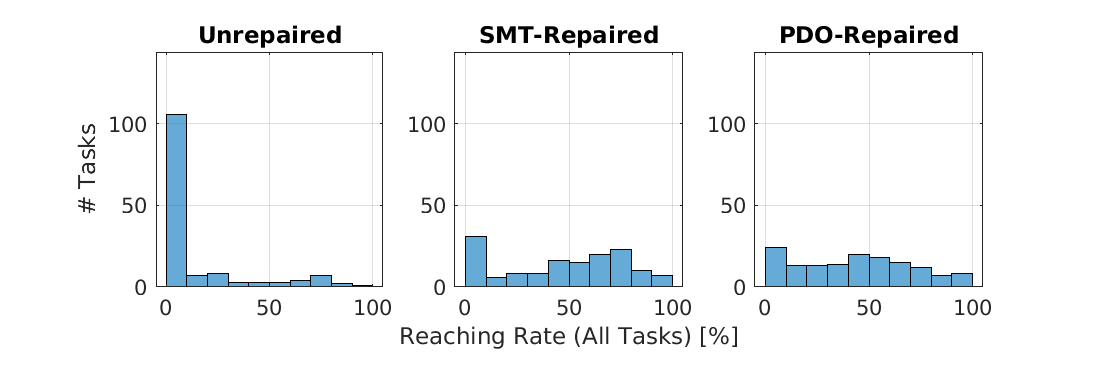
\includegraphics[width=\textwidth]{Images/second-experiment/exp1_RR_all_hist.eps}
    \caption{Histogram showing the number of successful tasks for Reaching Rate (RR) for the second experiment for the controllers of interest}
    \label{fig:hist-RR-all-second}
\end{figure}
As can be seen from image \ref{fig:box-RR-all-second} and tables \ref{tab:RR-all-second-cohen-p} and \ref{tab:RR-all-second-mean-std} even considering all the tasks together the reaching rates of the tasks executed on the two repaired controllers are higher then those of the task executed on the unrepaired one. There is a large effect size and an high statistical significance between the unrepaired controller and the repaired ones. As we could expect there is no significant difference between the two repaired controllers.
%
%
%
%
%
\subsubsection{Time to Complete Task (TCT)}\label{subsub:second-TCT}
As in the first experiment, we have decided to present the analysis of the TCTs both for only the successful tasks and for all the task together.
\begin{figure}[H]
    \centering
    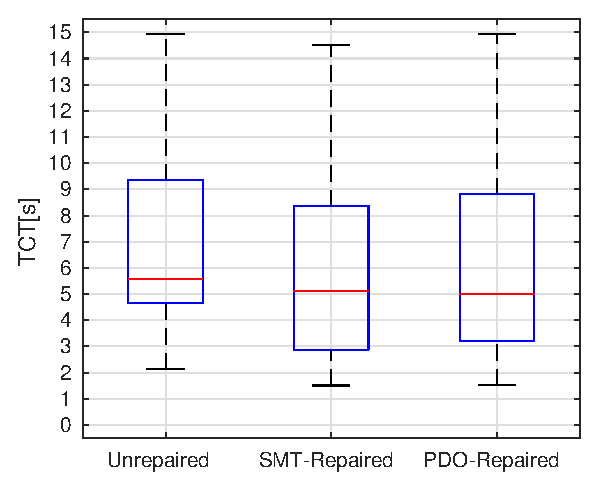
\includegraphics[width=\textwidth]{Images/second-experiment/exp1_TCT_succ.eps}
    \caption{Boxplot showing the Time to Complete Task (TCT) of the successful tasks of the second experiment for the controllers of interest}
    \label{fig:box-TCT-succ-second}
\end{figure}
\begin{table}[H]
    \centering
    \begin{tabular}{|c|c|c|c|}
        \hline
        - & \textbf{Unrepaired} & \textbf{SMT-Repaired} & \textbf{PDO-Repaired} \\
        \hline
        \textbf{Mean} & 7.0561s & 5.8643s & 5.9673s \\
        \textbf{Standard Deviation} & 4.0178s & 3.5300s & 3.5315s \\
        \hline
    \end{tabular}
    \caption{Table showing the mean and standard deviation of the Time to Complete Task for the successful tasks for the different controllers of interest in the second experiment.}
    \label{tab:TCT-succ-second-mean-std}
\end{table}
\begin{figure}[H]
    \centering
    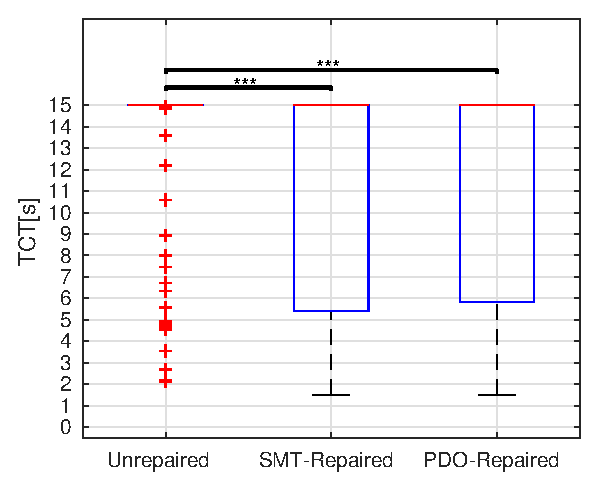
\includegraphics[width=\textwidth]{Images/second-experiment/exp1_TCT.eps}
    \caption{Boxplot showing the Time to Complete Task (TCT) of all the tasks of the second experiment for the controllers of interest}
    \label{fig:box-TCT-all-second}
\end{figure}
\begin{table}[H]
    \centering
    \begin{tabular}{|c|c|c|c|}
        \hline
        - & \textbf{Unrepaired} & \textbf{SMT-Repaired} & \textbf{PDO-Repaired} \\
        \hline
        \textbf{Mean} & 13.8456s & 10.7919s & 10.8626s \\
        \textbf{Standard Deviation} & 3.1911s & 5.1655s & 5.1076s \\
        \hline
    \end{tabular}
    \caption{Table showing the mean and standard deviation of the Time to Complete Task for the all the tasks for the different controllers of interest in the second experiment.}
    \label{tab:TCT-all-second-mean-std}
\end{table}
\begin{table}[H]
    \centering
    \begin{tabular}{|c|c|c|}
        \hline
        - & \textbf{Cohen's} $\mathbf{d}$ & $\mathbf{p-value}$ \\
        \hline
        \textbf{Unrepaired / SMT-Repaired} & 0.7206 & $4.3650 \cdot 10^{-8}$ \\
        \textbf{Unrepaired / PDO-Repaired} & 0.7005 & $7.5773 \cdot 10^{-9}$ \\
        \textbf{SMT-Repaired / PDO-Repaired} & 0.0216 & 0.6778 \\
        \hline
    \end{tabular}
    \caption{Table showing the Cohen's $d$ coefficient and the p-value of the Time to Complete Task for the different combinations of the controllers of interest in the second experiment.}
    \label{tab:TCT-all-second-cohen-p}
\end{table}
As can be seen from figure \ref{fig:box-TCT-succ-second} and table \ref{tab:TCT-succ-second-mean-std} there is not really a great difference between the TCTs of the successful tasks executed on the repaired controllers and those executed on the unrepaired one. The effect size and statistical significance which can be seen from figure \ref{fig:box-TCT-all-second} and table \ref{tab:TCT-all-second-cohen-p} are actually due to the higher number of successful task for the two repaired machine. Therefore the above mentioned results can be seen as a confirmation of what we have found in the Success Rate analysis.
%
%
%
%
%
\subsubsection{Time In Target (TIT)}\label{subsub:second-TIT}
As for the first experiment for the analysis of the TITs we decided to consider separately the analysis of the failed tasks and of all tasks.
\begin{figure}[H]
    \centering
    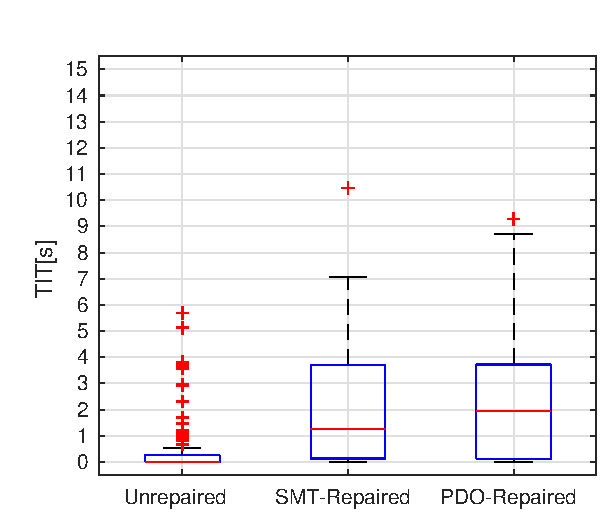
\includegraphics[width=\textwidth]{Images/second-experiment/exp1_TIT_fail.eps}
    \caption{Boxplot showing the Time In Target (TIT) of the failed tasks of the second experiment for the controllers of interest}
    \label{fig:box-TIT-fail-second}
\end{figure}
\begin{table}[H]
    \centering
    \begin{tabular}{|c|c|c|c|}
        \hline
        - & \textbf{Unrepaired} & \textbf{SMT-Repaired} & \textbf{PDO-Repaired} \\
        \hline
        \textbf{Mean} & 0.4542s & 2.1294s & 2.3013s \\
        \textbf{Standard Deviation} & 1.0810s & 2.3144s & 2.3686s \\
        \hline
    \end{tabular}
    \caption{Table showing the mean and standard deviation of the Time In Target for the failed tasks for the different controllers of interest in the second experiment.}
    \label{tab:TIT-fail-second-mean-std}
\end{table}
\begin{figure}[H]
    \centering
    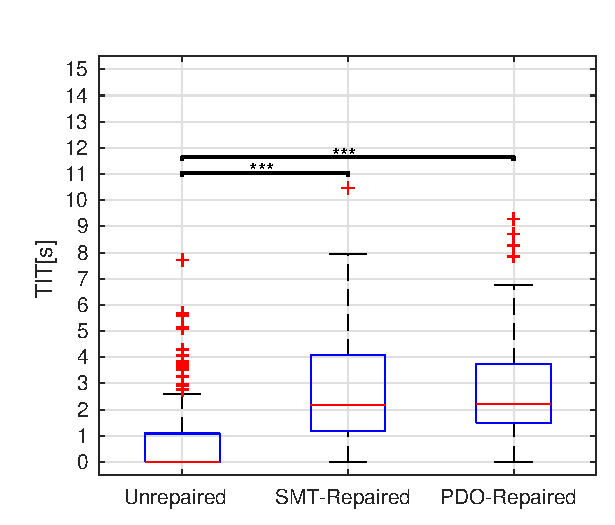
\includegraphics[width=\textwidth]{Images/second-experiment/exp1_TIT.eps}
    \caption{Boxplot showing the Time In Target (TIT) of all the tasks of the second experiment for the controllers of interest}
    \label{fig:box-TIT-all-second}
\end{figure}
\begin{table}[H]
    \centering
    \begin{tabular}{|c|c|c|c|}
        \hline
        - & \textbf{Unrepaired} & \textbf{SMT-Repaired} & \textbf{PDO-Repaired} \\
        \hline
        \textbf{Mean} & 0.8742s & 2.6000s & 2.5592s \\
        \textbf{Standard Deviation} & 1.5361s & 2.0876s & 2.0358s \\
        \hline
    \end{tabular}
    \caption{Table showing the mean and standard deviation of the Time In Target for the all the tasks for the different controllers of interest in the second experiment.}
    \label{tab:TIT-all-second-mean-std}
\end{table}
\begin{table}[H]
    \centering
    \begin{tabular}{|c|c|c|}
        \hline
        - & \textbf{Cohen's} $\mathbf{d}$ & $\mathbf{p-value}$ \\
        \hline
        \textbf{Unrepaired / SMT-Repaired} & 0.9416 & $1.4713 \cdot 10^{-13}$ \\
        \textbf{Unrepaired / PDO-Repaired} & 0.9344 & $2.6924 \cdot 10^{-12}$ \\
        \textbf{SMT-Repaired / PDO-Repaired} & 0.0198 & 0.9647 \\
        \hline
    \end{tabular}
    \caption{Table showing the Cohen's $d$ coefficient and the p-value of the Time In Target for the different combinations of the controllers of interest in the second experiment.}
    \label{tab:TIT-all-second-cohen-p}
\end{table}
From figures \ref{fig:box-TIT-fail-second} and \ref{fig:box-TIT-all-second} and tables \ref{tab:TIT-fail-second-mean-std}, \ref{tab:TIT-all-second-mean-std} and \ref{tab:TIT-all-second-cohen-p} the failed tasks of the repaired controllers present TITs higher then those of the unrepaired one. In particular we can see that there is a large effect size and an high statistical significance between the unrepaired controller and the repaired ones. As we expected there is not a significant difference between the two repaired controllers.
%
%
%
%
%
\subsubsection{Time To Repair (TTR)}\label{subsub:second-TTR}
\begin{figure}[H]
    \centering
    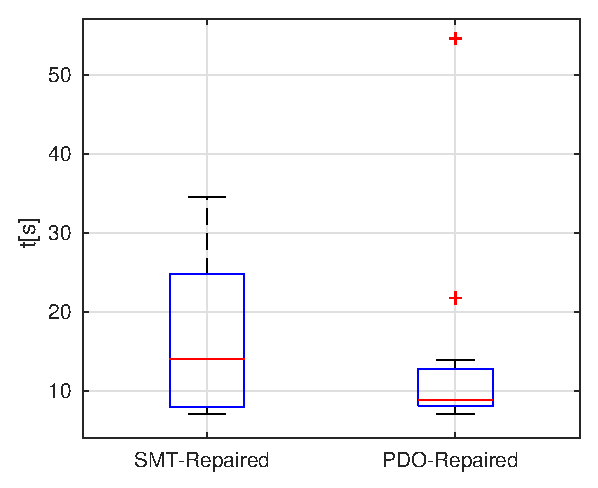
\includegraphics[width=\textwidth]{Images/second-experiment/exp1_time_to_repair.eps}
    \caption{Boxplot showing the Time To Repair (TTR) for all the participants of the second experiment for the controllers of interest}
    \label{fig:box-TTR-second}
\end{figure}
\begin{table}[H]
    \centering
    \begin{tabular}{|c|c|c|}
        \hline
        - & \textbf{SMT-Repaired} & \textbf{PDO-Repaired} \\
        \hline
        \textbf{Mean} & 16.6998s & 14.1202s \\
        \textbf{Standard Deviation} & 10.0184s & 13.4058s \\
        \hline
    \end{tabular}
    \caption{Table showing the mean and standard deviation of the Time To Repair for the all the participants for the different controllers of interest in the second experiment.}
    \label{tab:TTR-second-mean-std}
\end{table}
\begin{table}[H]
    \centering
    \begin{tabular}{|c|c|c|}
        \hline
        - & \textbf{Cohen's} $\mathbf{d}$ & $\mathbf{p-value}$ \\
        \hline
        \textbf{SMT-Repaired / PDO-Repaired} & 0.2180 & 0.3013 \\
        \hline
    \end{tabular}
    \caption{Table showing the Cohen's $d$ coefficient and the p-value of the Time To Repair for the different combinations of the controllers of interest in the second experiment.}
    \label{tab:TTR-second-cohen-p}
\end{table}
As can be seen from image \ref{fig:box-TTR-second} and tables \ref{tab:TTR-second-mean-std} and \ref{tab:TTR-second-cohen-p} the result we have found in the second experiment are not consistent with what we have found in the first experiment. This can be due to some problem on the computer which executed the repair process for the two participants corresponding to the two outliers that can be seen in figure \ref{fig:box-TTR-second} for the PDO repaired controller.\\\\
As last remark, the high variance of the performance measures we have considered in the previous analysis is due to the high variance between the characteristic of the participants: based on the muscular configuration of the participant the reading of the sEMG signals can change, therefore making the distinction between different action easier or harder.